\chapter{الحيوانات عبر فصول السنة}\label{ch:g3:animals-through-seasons}

في تشرين الأول تصطف السنونوات على الأسلاك، وفي صباح من الأيام
تختفي. والقنفذ تحت السياج يلفّ نفسه في عشه الورقي فلا يُرى قبل
الربيع. أما الثعلب فهو في الخارج في كل ثلج. الشتاء موسم قاسٍ ---
بارد، وقليل الغذاء قبل كل شيء --- وللحيوانات ثلاث طرق كبرى
لعبوره.

\section{الشتاء موسم الشحّ}

\begin{proposition}[مشكلة الشتاء المزدوجة]\label{prop:g3:animals-through-seasons:problem}
يجلب الشتاء \omterm{def:g1:animals-around-us:animal}{للحيوانات} مشكلتين معًا:
\begin{enumerate}
  \item \emph{البرد}، وهو يستنزف دفء الجسم أسرع --- والبقاء
        دافئًا يكلّف \omterm{prop:g3:balanced-diet:jobs}{طاقة}
        (\cref{prop:g3:balanced-diet:jobs})؛
  \item و\emph{شحّ الغذاء}: \omterm{def:g1:plants-around-us:plant}{فالنباتات} تكفّ عن النمو، \omterm{prop:g3:sorting-living-things:groups}{والحشرات}
        تختفي، وتنحل الحلقات الأولى من \omterm{def:g3:food-chains:chain}{السلاسل الغذائية} في
        \cref{ch:g3:food-chains} --- فيسري الشحّ صعودًا إلى
        الجميع.
\end{enumerate}
دفء أكثر مطلوب، وغذاء أقل لدفع ثمنه: تلك هي مشكلة الشتاء التي على
كل \omterm{def:g1:animals-around-us:animal}{حيوان} أن يحلّها.
\end{proposition}
\admitted

\begin{example}[أين ذهب غذاء آكلات الحشرات؟]\label{ex:g3:animals-through-seasons:insects}
السنونو يتغذى على \omterm{prop:g3:sorting-living-things:groups}{الحشرات} الطائرة، يمسكها في الجو. وفي تشرين
الثاني لا يوجد منها شيء ببساطة: فالبرد شديد. ولا تبديل للمائدة
يصلح ذلك لطائر مبني للصيد الجوي --- فمورد غذاء السنونو يزول تمامًا.
\end{example}

\begin{omfigure}
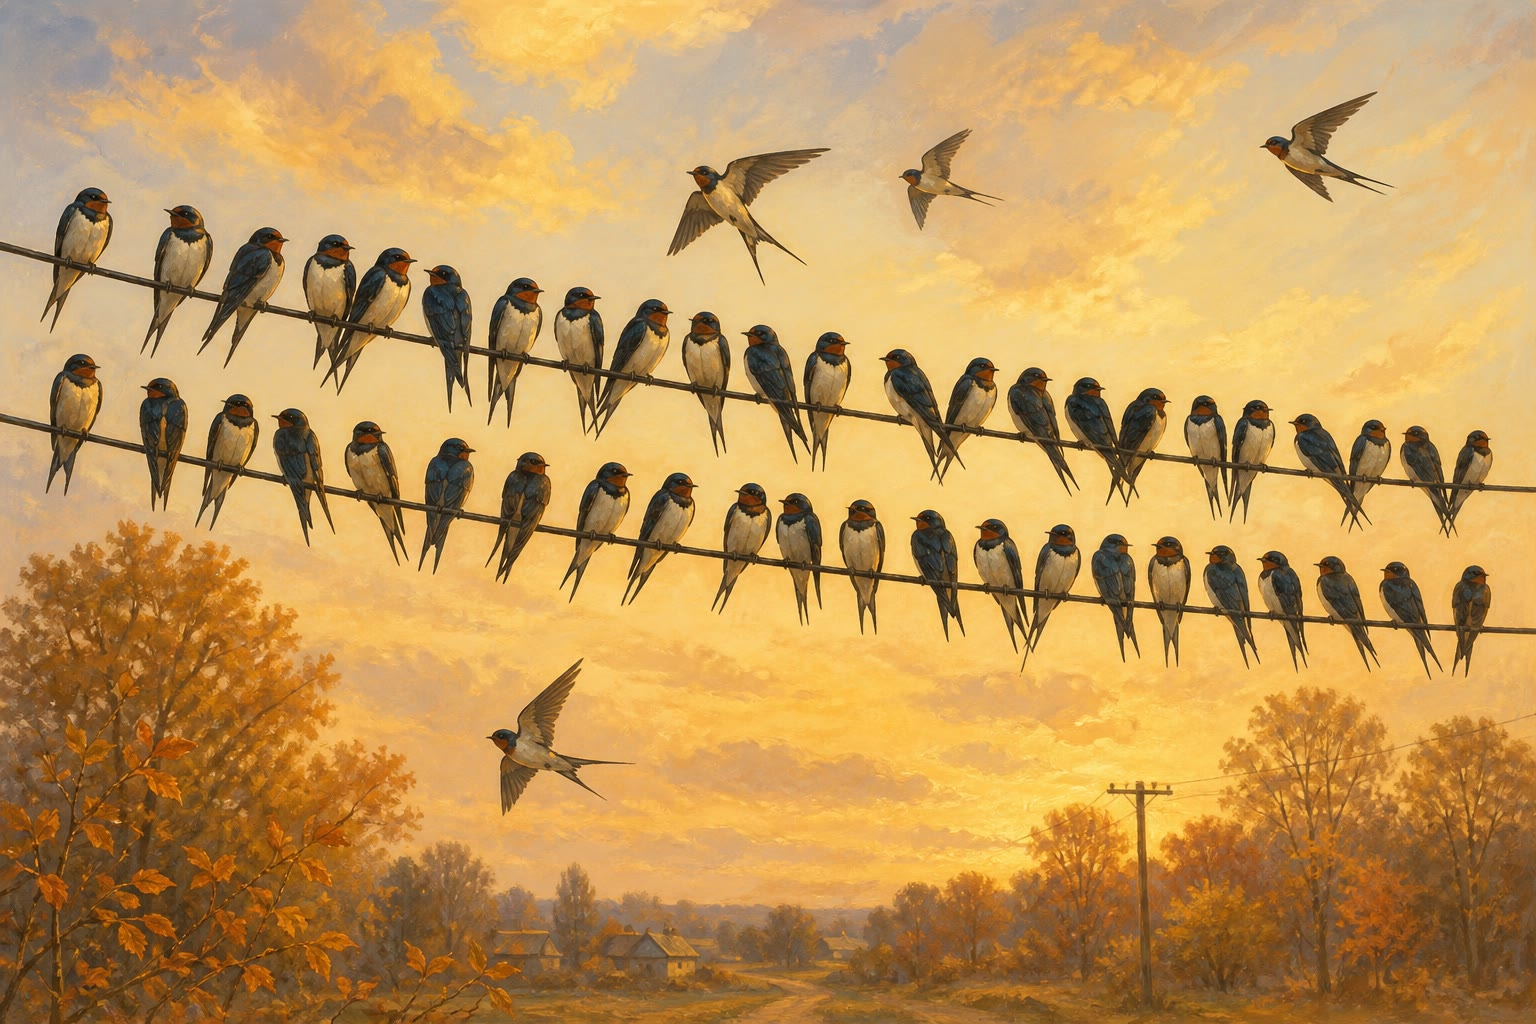
\includegraphics[width=0.62\linewidth]{images/book1/ai/g3-seasons-swallows.jpg}

{\small تشرين الأول على الأسلاك: السنونوات تتجمع للرحيل، قبل أيام
من نفاد \omterm{prop:g3:sorting-living-things:groups}{الحشرات}.}
\end{omfigure}

\section{ثلاثة أجوبة عن الشتاء}

\begin{definition}[الهجرة]\label{def:g3:animals-through-seasons:migration}
أن \emph{يهاجر}\index{هجرة} \omterm{def:g1:animals-around-us:animal}{الحيوان} هو أن يرتحل كل سنة من إقليم
إلى آخر مع تغير فصول السنة --- فيغادر قبل الشتاء إلى بلاد أدفأ
يبقى فيها الغذاء، ويعود في الربيع. والسنونو واللقلق والكركي
\emph{طيور مهاجرة}\index{مهاجر}؛ ويقطع بعضها آلاف الكيلومترات،
ويهتدي إلى العش نفسه بعينه.
\end{definition}

\begin{definition}[السبات الشتوي]\label{def:g3:animals-through-seasons:hibernation}
أن \emph{يسبت}\index{سبات} \omterm{def:g1:animals-around-us:animal}{الحيوان} هو أن يقضي الشتاء في \omterm{prop:g1:healthy-habits:needs}{نوم} عميق
بارد، مختبئًا في مأوى: فيبرد الجسم، ويبطؤ القلب والتنفس حتى
يكادان يقفان، ويعيش \omterm{def:g1:animals-around-us:animal}{الحيوان} ببطء على شحم ادّخره في الخريف. والقنفذ
والزغبة والغرير الجبلي والخفاش تسبت.
\end{definition}

\begin{definition}[البقاء نشطًا]\label{def:g3:animals-through-seasons:active}
أما البقية فتبقى \emph{نشطة}\index{البقاء نشطًا في الشتاء}
وتغيّر عتادها أو عاداتها: \emph{فروة شتوية}\index{فروة شتوية}
أكثف، و\emph{مخازن غذاء}\index{مخزن غذاء} تُجمع في الخريف
(كجوز السنجاب المدفون)، أو تبديل للمائدة
(كشحرور \cref{ex:g2:what-animals-eat:winter})، أو مجرد بحث أشقّ
--- كالثعلب والأيّل وأبي الحنّاء.
\end{definition}

\begin{omfigure}
\begin{tikzpicture}
  \draw[thick, omDef, fill=omDef!7, rounded corners=6pt]
    (0,0) rectangle (4.1,3.1);
  \draw[thick, omProp, fill=omProp!7, rounded corners=6pt]
    (4.5,0) rectangle (8.6,3.1);
  \draw[thick, omMeth, fill=omMeth!7, rounded corners=6pt]
    (9.0,0) rectangle (13.1,3.1);
  \node[font=\small\bfseries, omDef, text height=1.6ex, text depth=0.4ex]
    at (2.05,2.75) {هجرة};
  \node[font=\small\bfseries, omProp, text height=1.6ex, text depth=0.4ex]
    at (6.55,2.75) {سبات};
  \node[font=\small\bfseries, omMeth, text height=1.6ex, text depth=0.4ex]
    at (11.05,2.75) {بقاء نشطًا};
  \node[font=\small, align=center, text width=3.8cm] at (2.05,1.2)
    {الرحيل إلى بلاد\\ يبقى فيها الغذاء\\[2pt] سنونو، ولقلق،\\ وكركي};
  \node[font=\small, align=center, text width=3.8cm] at (6.55,1.2)
    {نوم عميق بارد،\\ عيشًا على الشحم المدّخر\\[2pt] قنفذ، وغرير جبلي،\\ وزغبة، وخفاش};
  \node[font=\small, align=center, text width=3.8cm] at (11.05,1.2)
    {فروة شتوية، ومخازن،\\ ومائدة جديدة، وبحث شاق\\[2pt] ثعلب، وسنجاب،\\ وأبو حنّاء، وأيّل};
\end{tikzpicture}

{\small ثلاث طرق عبر الشتاء نفسه. وكل واحدة تحلّ المشكلة المزدوجة
--- الدفء والغذاء --- على نحو مختلف.}
\end{omfigure}

\begin{example}[ثلاثة جيران وثلاث خطط]\label{ex:g3:animals-through-seasons:three}
سياج نباتي واحد في كانون الثاني: السنونوات التي عشّشت فوقه في
إفريقيا تمسك \omterm{prop:g3:sorting-living-things:groups}{الحشرات} تحت شمس دافئة؛ والقنفذ تحته ينام باردًا
بطيئًا في عشه الورقي، يحرق شحم آب؛ وأبو الحنّاء فوقه، في ريشه
الشتوي المنفوش، يجوب باحثًا عن آخر التوت. وفي نيسان يعود الثلاثة
جميعًا إلى العمل في السياج نفسه.
\end{example}

\begin{remark}[النوم ليس كسلًا، والسفر ليس سياحة]\label{rem:g3:animals-through-seasons:cost}
لكل خطة ثمنها. \omterm{def:g3:animals-through-seasons:migration}{فالمهاجر} يخاطر برحلة منهكة؛ والسابت عليه أن يجمع
كل غرام من شحم شتائه في الخريف --- والقنفذ النحيل في تشرين الثاني
لن يستيقظ في الربيع؛ \omterm{def:g1:animals-around-us:animal}{والحيوان} النشط يقامر على إيجاد الغذاء عبر
أجوع الشهور. فثمن الشتاء يُدفع سلفًا، أو في الطريق، أو يومًا بيوم.
\end{remark}

\begin{method}[تخمين خطة حيوان في الشتاء]\label{met:g3:animals-through-seasons:guess}
\begin{enumerate}
  \item اسأل ماذا يأكل، وأيوجد ذلك الغذاء هنا في الشتاء؛
  \item فإن كان الغذاء قد زال تمامًا (\omterm{prop:g3:sorting-living-things:groups}{كالحشرات} الطائرة والرحيق):
        فتوقّع \omterm{def:g3:animals-through-seasons:migration}{هجرة} أو سباتًا؛
  \item وإن كان الغذاء ممكن الإيجاد (\omterm{def:g2:from-seed-to-plant:seed}{كالبذور} والتوت والفريسة):
        فتوقّع شتاءً نشطًا، وربما بفروة أكثف أو بمخازن؛
  \item وراجع في الخريف: فالتسمين وحفر العش يدلان على \omterm{def:g3:animals-through-seasons:hibernation}{السبات}؛
        والتجمع في أسراب يدل على الرحيل.
\end{enumerate}
\end{method}

\begin{example}[الربيع ينقض ذلك كله]\label{ex:g3:animals-through-seasons:spring}
في آذار ونيسان ينعكس الترتيب: فتعود \omterm{prop:g3:sorting-living-things:groups}{الحشرات}، ويظهر المهاجرون من
جديد عند أعشاشهم القديمة، ويستيقظ السابتون نحافًا جائعين، وتُطرح
الفروات الشتوية. تدور فصول السنة، ويدور معها تقويم \omterm{def:g1:animals-around-us:animal}{الحيوانات} ---
وفي الخريف القادم تصطف السنونوات على الأسلاك من جديد.
\end{example}

\section{تمارين}

\begin{exercise}[$\star$]\label{exo:g3:animals-through-seasons:1}
ما المشكلة المزدوجة التي يضعها الشتاء أمام كل \omterm{def:g1:animals-around-us:animal}{حيوان}؟
\end{exercise}

\begin{exercise}[$\star$]\label{exo:g3:animals-through-seasons:2}
سمِّ خطط الشتاء الثلاث، مع حيوانين لكل واحدة.
\end{exercise}

\begin{exercise}[$\star$]\label{exo:g3:animals-through-seasons:3}
ماذا يحدث لجسم القنفذ السابت في أثناء نومه الطويل؟ وعلام يعيش؟
\end{exercise}

\begin{exercise}[$\star$]\label{exo:g3:animals-through-seasons:4}
لماذا يجب على السنونو أن يرحل بالضبط --- ما غذاؤه، وماذا يصير له
هنا في الشتاء؟
\end{exercise}

\begin{exercise}[$\star$]\label{exo:g3:animals-through-seasons:5}
اذكر ثلاث طرق يعبر بها \omterm{def:g1:animals-around-us:animal}{حيوان} نشط الشتاء، مع \omterm{def:g1:animals-around-us:animal}{حيوان} لكل واحدة.
\end{exercise}

\begin{exercise}[$\star$]\label{exo:g3:animals-through-seasons:6}
ما ثمن كل خطة، وفق \cref{rem:g3:animals-through-seasons:cost}؟
\end{exercise}

\begin{exercise}[$\star$]\label{exo:g3:animals-through-seasons:7}
في الخريف يُرى \omterm{def:g1:animals-around-us:animal}{حيوان} يأكل بنهم ويبطّن حفرة \omterm{def:g1:plants-around-us:parts}{بأوراق} يابسة. فأي خطة
يهيّئ؟ وأي خطوة من \cref{met:g3:animals-through-seasons:guess}
دلّتك؟
\end{exercise}

\begin{exercise}[$\star$]\label{exo:g3:animals-through-seasons:8}
جرّب: احتفظ بقائمة شتوية للطيور التي تراها فعلًا في الخارج خلال
أسبوع بارد. أفي القائمة سنونوات؟ وأي طيورك اختارت خطة البقاء
\omterm{def:g3:animals-through-seasons:active}{نشطة}؟
\end{exercise}

\begin{exercise}[$\star\star$]\label{exo:g3:animals-through-seasons:9}
استعمل \cref{met:g3:animals-through-seasons:guess} على: (أ)
السنجاب (يأكل الجوز \omterm{def:g2:from-seed-to-plant:seed}{والبذور})؛ (ب) الكركي (يأكل ضفادع وحشرات
المروج الرطبة). فماذا يفعل كل واحد في الشتاء على الأرجح؟
\end{exercise}

\begin{exercise}[$\star\star$]\label{exo:g3:animals-through-seasons:10}
خريف معتدل يبقي قنفذًا صغيرًا يقظًا يصطاد متأخرًا، لكنه يبقى
نحيلًا. فلماذا كان هذا خطرًا عليه وفق
\cref{rem:g3:animals-through-seasons:cost}؟ وماذا يفعل منقذو
\omterm{def:g1:animals-around-us:animal}{الحيوانات} بقنافذ الخريف النحيلة؟
\end{exercise}
